\documentclass[twoside,11pt]{article}

\usepackage{../Style/feuille-tp}

\formation{IUT - Département Informatique}
\matiere{Théorie des langages}
\titre{Devoir Surveillé}
\sigle{Maths \\ 2013-2014}


\sloppy

\begin{document}


\maketitle

\textbf{Sans documents, durée 1h30}

\begin{multicols*}{2}
\section{Grammaires algébriques}

\Q Soit la grammaire $\mathcal{G}$ ci dessous, d'axiome $S$ 
$$\begin{array}{|rcl|rcl|}
S & \rightarrow &a S a &
T & \rightarrow & b T b  \\
S & \rightarrow & T & 
T & \rightarrow & \epsilon 
\end{array}
$$
\begin{enumerate}
\item Dessinez l'arbre de dérivation du mot $aabbaa$.
\item Quel est le langage engendré par $\mathcal{G}$ ?
\end{enumerate}

\Q Les \textbf{palindromes} sont des mots qui se lisent
de la même façon dans les 2 sens).  Par exemple
$\epsilon, aaa, abba, aaabbaaa$ sont des palindromes.
\begin{enumerate}
\item Donnez une grammaire pour les palindromes sur
$A = \{a,b\}$
\item Montrez l'arbre de dérivation du mot $babab$.
\end{enumerate}

\Q Dans le manuel d'un langage de programmation, la syntaxe des 
\emph{instructions}  est définie ainsi
\begin{center}
\begin{tabular}{|rcl|}
\hline
Instr. & $\rightarrow$ &\underline{si} Cond.
\underline{alors} Instr. \\  
Instr. & $\rightarrow$ &\underline{si} Cond.
\underline{alors} Instr. 
\underline{sinon} Instr.  \\  
Instr. & $\rightarrow$ & Affect. \\
$\ldots$ &&
\\ \hline

\end{tabular}
\end{center}
à partir des conditions, des affectations etc.
\begin{enumerate}
\item Montrez que cette grammaire est ambigüe
\item Proposez une modification du langage pour éviter ce problème.
\end{enumerate}

\Q Soit $\mathcal{G}_1$, $\mathcal{G}_2$ les grammaires - d'axiomes
respectifs - $S_1$ et $ S_2$, qui reconnaissent deux langages
algébriques $L_1$ et $L_2$.  Montrez comment, en y ajoutant un axiome
$S$ et quelques règles, on peut construire des grammaires pour :
\begin{enumerate}
\item le produit par concaténation $L_1  L_2$,
\item l'union $L_1 + L_2$,
\item l'étoile $L_1^*$.
\end{enumerate}


\section{Langages rationnels}


\Q Donnez un automate déterministe sur l'alphabet $A = \{a, b, c\}$
 qui reconnaisse le langage
$L_1$ des mots qui commencent par le préfixe $ab$.

\Q Même question pour 
$L_2$, les mots qui finissent par le suffixe $bc$.

\Q Expliquez comment construire un automate qui reconnait l'intersection
de deux langages rationnels, en l'illustrant sur le cas de  $L_1 \cap L_2$.

\section{Expressions régulières}


\Q  Par définition, l'étoile de Kleene d'un langage $L$ est 
$$L^* = \epsilon + L + L^2 + L^3 + \ldots$$
Prouvez que pour tout $L$ :
\begin{eqnarray}
L^* &=& \epsilon + L L^* \\
L^* L^* &=& L^* \\
{(L^*)}^*  &=&  L^*
\end{eqnarray}



\Q Est-ce que $ (L_1 + L_2)^*  = L_1^* + L_2^* $ ? (justifiez).

\Q Soit $\mathcal{A}$ l'automate non-déterministe ci-dessous, où
l'état 0 est initial, et 3 est final.
\begin{center}
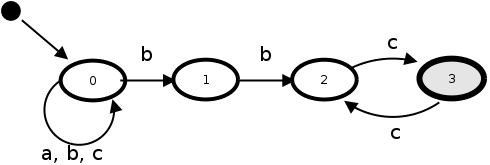
\includegraphics[width=\linewidth]{../dia/bbc}
\end{center}
\begin{enumerate}
\item Quelles équations entre le langage $L$ reconnu par $\mathcal{A}$
et $L_0, L_1, \ldots$ (liés aux états).
\item En déduire une expression régulière pour $L$.
\end{enumerate}
% \Q Appliquez la procédure de déterminisation.

\end{multicols*}

\end{document}

